\chapter{Stochastic and Deterministic Processes}

\begin{refsection}

\section{Stochastic Processes}

\begin{itemize}
	\item Stochastic processes $\rightarrow$ random signal
	\item No deterministic description
	\item Description of random parameters (probability, ...)
\end{itemize}

\subsection{Statistic Mean}

Given is family of curves $\vect{x}(t) = \left\{x_1(t), x_2(t), \dots, x_n(t)\right\}$:

\begin{figure}[H]
	\centering
	\begin{tikzpicture}
		\begin{axis}[
			height={0.25\textheight},
			width=0.6\linewidth,
			scale only axis,
			xlabel={$t$},
			ylabel={$x(t)$},
			%grid style={line width=.6pt, color=lightgray},
			%grid=both,
			grid=none,
			legend pos=north east,
			axis y line=middle,
			axis x line=middle,
			every axis x label/.style={
				at={(ticklabel* cs:1.05)},
				anchor=north,
			},
			every axis y label/.style={
				at={(ticklabel* cs:1.05)},
				anchor=east,
			},
			xmin=0,
			xmax=11,
			ymin=0,
			ymax=1.7,
			xtick={0, 1, ..., 10},
			ytick={0, 0.5, ..., 1.5},
			xticklabels={0, 1, $t_0$, 3, 4, ..., 10}
		]
			\addplot[black, dashed, smooth, domain=1:10, samples=200] plot (\x,{1.5*abs(sinc((1/(2*pi))*\x))});
			\pgfmathsetseed{100}
			\addplot[red, smooth, domain=1:10, samples=50] plot (\x,{1.5*abs(sinc((1/(2*pi))*\x)) + 0.1*rand});
			\addlegendentry{$x_1$};
			\pgfmathsetseed{200}
			\addplot[blue, smooth, domain=1:10, samples=50] plot (\x,{1.5*abs(sinc((1/(2*pi))*\x)) + 0.1*rand});
			\addlegendentry{$x_2$};
			\pgfmathsetseed{300}
			\addplot[green, smooth, domain=1:10, samples=50] plot (\x,{1.5*abs(sinc((1/(2*pi))*\x)) + 0.1*rand});
			\addlegendentry{$x_3$};
			\addplot[black, very thick, dashed] coordinates {(2,0) (2,2.2)};
		\end{axis}
	\end{tikzpicture}
	\caption{Family of random signals}
\end{figure}

\begin{itemize}
	\item The curves are produced by a random process $\vect{x}(t)$. The random process is time-dependent.
	\item All curves consist of random values, which are gathered around a mean value $\E\left\{\vect{x}(t)\right\}$.
	\item The random process can emit any value $x$. However, each value $x$ has a certain probability $p(x, t)$. Again, the probability is time-dependent like the stochastic process.
\end{itemize}

Let's assume that the values are normally distributed. The \index{probability density function} \textbf{\ac{PDF}} $p(x, t)$ of a \index{normal distribution} \textbf{normal distribution} is:
\begin{equation}
	p(x, t) = \frac{1}{\sigma(t) \sqrt{2 \pi}} e^{-\frac{1}{2} \left(\frac{x - \mu(t)}{\sigma(t)}\right)^2}
\end{equation}
$p(x, t)$ is the probability that the stochastic process emits the value $x$ at time instance $t$. Both the mean of the normal distribution $\mu(t)$ and the standard deviation of the normal distribution $\sigma(t)$ are time-dependent.

\begin{attention}
	Do not confuse the mean of the normal distribution $\mu$ and the mean of a series of samples $\E\left\{\cdot\right\}$ (expectation value)!
\end{attention}

\begin{figure}[H]
	\centering
	\begin{tikzpicture}
		\begin{axis}[
			height={0.25\textheight},
			width=0.8\linewidth,
			scale only axis,
			xlabel={$x$},
			ylabel={$p(x, t_0)$},
			%grid style={line width=.6pt, color=lightgray},
			%grid=both,
			grid=none,
			legend pos=north east,
			axis y line=middle,
			axis x line=middle,
			every axis x label/.style={
				at={(ticklabel* cs:1.05)},
				anchor=north,
			},
			every axis y label/.style={
				at={(ticklabel* cs:1.05)},
				anchor=east,
			},
			xmin=-1.2,
			xmax=4.2,
			ymin=0,
			ymax=1.2,
			xtick={-1, 0, 1, 1.47, 2, 3, 4},
			ytick={0, 0.5, ..., 2.0},
			xticklabels={-1, 0, 1, $\E\left\{\vect{x}(t_0)\right\}$, 2, 3, 4}
		]
			% µ = 1.47, simga = 0.5
			\addplot[red, thick, smooth, domain=, samples=200] plot (\x, {(1/(0.5*sqrt(2*pi)))*exp(-0.5*((\x-1.47)/0.5)^2)});
			
			\addplot[black, very thick, dashed] coordinates {(1.47,0) (1.47,1)};
		\end{axis}
	\end{tikzpicture}
	\caption{Probability for an output value of a stochastic process at time $t_0$ with $\mu(t_0) = 1.47$ and $\sigma(t_0) = 0.5$}
\end{figure}

Given that
\begin{itemize}
	\item We know neither the mean of the normal distribution $\mu(t)$ nor the standard deviation of the normal distribution $\sigma(t)$.
	\item We only have $n$ samples of the curves $x_i(t_0)$ ($i \in \mathbb{N}, 0 \leq i \leq n$) at the time instance $t_0$.
	\item We do know that the random distribution of our samples $x_i(t_0)$ follows the \ac{PDF} $p(x, t_0)$.
\end{itemize}

\paragraph{How do we get the mean of out samples $\E\left\{X(t_0)\right\}$? (Finite case)}

The mean of the samples is the \index{expectation value} \textbf{expectation value} $\E\left\{\vect{x}(t_0)\right\}$. \nomenclature[Se]{$\E\left\{\cdot\right\}$}{Expectation value}

To get an approximation, we can calculate the \index{arithmetic mean} \textbf{arithmetic mean} of out $n$ samples:
\begin{equation}
	\E\left\{\vect{x}(t_0)\right\} \approx \frac{1}{n} \sum\limits_{i = 0}^{n} x_i(t_0)
	\label{eq:ch03:arith_mean}
\end{equation}
The approximation converges to the real $\E\left\{\vect{x}(t_0)\right\}$ for $n \rightarrow \infty$, because the random distribution of our samples $x_i(t_0)$ follows the \ac{PDF} $p(x, t_0)$.

\paragraph{What about an arbitrary \ac{PDF}? (Continuous case)}

\begin{itemize}
	\item We cannot collect an indefinite number of samples.
	\item However, if the \ac{PDF} is known, we can calculate the mean of our samples.
\end{itemize}

Extending, the arithmetic mean \eqref{eq:ch03:arith_mean}, with $n \rightarrow \infty$ and using all $x$ but weighted by their \ac{PDF} $p(x, t_0)$, we can determine the expectation value.
\begin{definition}{Stochastic mean}
	The \index{stochastic mean} \textbf{stochastic mean} of a \ac{PDF} is:
	\begin{equation}
		\E\left\{\vect{x}(t_0)\right\} = \int\limits_{-\infty}^{\infty} x \cdot p(x, t_0) \; \mathrm{d} x
	\end{equation}%
	\nomenclature[Se]{$\E\left\{\vect{x}\right\}$}{Stochastic mean}
\end{definition}

\begin{fact}
	In general, stochastic means are time-dependent.
\end{fact}

\paragraph{Other measures?}

The \index{quadratic stochastic mean} \textbf{quadratic stochastic mean}:
\begin{equation}
	\E\left\{\vect{x}^2(t_0)\right\} = \int\limits_{-\infty}^{\infty} x^2 \cdot p(x, t_0) \; \mathrm{d} x
\end{equation}

\subsection{Temporal Mean}

Given is a random time-domain signal $x_i(t)$ (where $i \in \mathbb{N}$ an arbitrary integer index):

\begin{figure}[H]
	\centering
	\begin{tikzpicture}
		\begin{axis}[
			height={0.25\textheight},
			width=0.6\linewidth,
			scale only axis,
			xlabel={$t$},
			ylabel={$x_i(t)$},
			%grid style={line width=.6pt, color=lightgray},
			%grid=both,
			grid=none,
			legend pos=north east,
			axis y line=middle,
			axis x line=middle,
			every axis x label/.style={
				at={(ticklabel* cs:1.05)},
				anchor=north,
			},
			every axis y label/.style={
				at={(ticklabel* cs:1.05)},
				anchor=east,
			},
			xmin=-5.5,
			xmax=5.5,
			ymin=0,
			ymax=3.2,
			xtick={-5, -4, ..., 5},
			ytick={0, 1, ..., 3},
			xticklabels={-5, -4, -3, -2, $-\frac{T}{2}$, 0, $\frac{T}{2}$, 2, 3, 4, 5}
		]
			\pgfmathsetseed{100}
			\addplot[red, smooth, domain=-5:5, samples=50] plot (\x,{1.5 + 0.8*rand});
			\addplot[black, thick, dashed] coordinates {(-1,0) (-1,3.2)};
			\addplot[black, thick, dashed] coordinates {(1,0) (1,3.2)};
			\addplot[black, dashed] coordinates {(-5,1.5) (5,1.5)};
		\end{axis}
	\end{tikzpicture}
	\caption{Random time-domain signal}
\end{figure}

\textit{Remark:} The signal can be a sample of a family of signals, but it is not required to be.

The temporal mean is calculated as the arithmetic mean with following differences to \eqref{eq:ch03:arith_mean}:
\begin{itemize}
	\item The mean is calculation over the time, not over a number of samples.
	\item For a time-continuous signal, the sum extends to an integral.
	\item The arithmetic mean is calculated over the time interval $[-\frac{T}{2}, \frac{T}{2}]$. Let's make the interval indefinite.
\end{itemize}

\begin{definition}{Temporal mean}
	The \index{temporal mean} \textbf{temporal mean} of time-domain signal $x_i(t)$ is:
	\begin{equation}
		\overline{x_i} = \E\left\{x_i(t)\right\} = \lim\limits_{T \rightarrow \infty} \frac{1}{T} \int\limits_{-\frac{T}{2}}^{\frac{T}{2}} x_i{t} \; \mathrm{d} t
	\end{equation}%
	\nomenclature[Sx]{$\overline{x}$, $\E\left\{x_i(t)\right\}$}{Temporal mean}
\end{definition}

The temporal mean is not time-dependent.

\begin{fact}
	In general, temporal means are sample-dependent.
\end{fact}

Actually $x_i(t)$ would not need the index $i$ if there is only one sample. Nevertheless, it was kept here, to emphasize the dependency on the sample, in contrast to the dependency on the time of the stochastic mean.

\paragraph{Other measures?}

The \index{quadratic temporal mean} \textbf{quadratic temporal mean}:
\begin{equation}
	\overline{x^2_i} = \E\left\{x^2_i(t)\right\} = \lim\limits_{T \rightarrow \infty} \frac{1}{T} \int\limits_{-\frac{T}{2}}^{\frac{T}{2}} |x_i{t}|^2 \; \mathrm{d} t
\end{equation}

\subsection{Ergodic Processes}

\begin{definition}{Ergodic process}
	\index{ergodic process} A process is \textbf{ergodic} if:
	\begin{enumerate}
		\item The stochastic means are equal at all times.
		\begin{equation}
			\E\left\{\vect{x}(t_0)\right\} = \E\left\{\vect{x}(t_1)\right\} = \dots = \E\left\{\vect{x}\right\}
		\end{equation}
		\item The temporal means of all samples are equal.
		\begin{equation}
			\overline{x_1} = \overline{x_2} = \dots = \overline{x}
		\end{equation}
		\item The stochastic mean equals the temporal mean.
		\begin{equation}
			\E\left\{\vect{x}\right\} = \overline{x} = \mu_x
		\end{equation}
	\end{enumerate}
\end{definition}

As a consequence:
\begin{itemize}
	\item One single, sufficiently long, random sample of the process is enough to deduct the statistical properties of an ergodic process.
	\item The ergodic process is in steady state, i.e., it does not erratically change its behaviour and properties.
\end{itemize}

\begin{figure}[H]
	\centering
		\begin{tikzpicture}
			\begin{axis}[
			height={0.25\textheight},
			width=0.6\linewidth,
			scale only axis,
			xlabel={$t$},
			ylabel={$x_i(t)$},
			%grid style={line width=.6pt, color=lightgray},
			%grid=both,
			grid=none,
			legend pos=north east,
			axis y line=middle,
			axis x line=middle,
			every axis x label/.style={
				at={(ticklabel* cs:1.05)},
				anchor=north,
			},
			every axis y label/.style={
				at={(ticklabel* cs:1.05)},
				anchor=east,
			},
			xmin=-5.5,
			xmax=5.5,
			ymin=0,
			ymax=3.2,
			xtick={-5, -4, ..., 5},
			ytick={0, 1, ..., 3},
			xticklabels={-5, -4, -3, -2, $-\frac{T}{2}$, 0, $\frac{T}{2}$, 2, 3, 4, 5}
			]
			\pgfmathsetseed{100}
			\addplot[red, smooth, domain=-5:5, samples=50] plot (\x,{1.5 + 0.8*rand});
			\addlegendentry{$x_1$};
			\pgfmathsetseed{200}
			\addplot[blue, smooth, domain=-5:5, samples=50] plot (\x,{1.5 + 0.8*rand});
			\addlegendentry{$x_2$};
			\pgfmathsetseed{300}
			\addplot[green, smooth, domain=-5:5, samples=50] plot (\x,{1.5 + 0.8*rand});
			\addlegendentry{$x_3$};
			\addplot[black, dashed] coordinates {(-5,1.5) (5,1.5)};
			\addlegendentry{$\mu_x$};
		\end{axis}
		\end{tikzpicture}
	\caption{Three samples of the same ergodic process}
\end{figure}

\subsection{Cross-Correlation}

\section{Spectral Density}

\subsection{Autocorrelation}

\subsection{Energy and Power Spectral Density}

\subsection{Decibel}

\section{Noise}

\subsection{Types of Noise}

\subsection{Thermal Noise}

\subsection{White Noise}

\subsection{Noise Floor and Noise Figure}

\phantomsection
\addcontentsline{toc}{section}{References}
\printbibliography[heading=subbibliography]
\end{refsection}

